% !TeX root = ../../tfg.tex
% !TeX encoding = utf8
%
%***************************************************************
% Contenido del artículo 5: Generalización a multi-output 
%***************************************************************
\section{Generalización para \textit{multi-output neuronal networks}}

En las secciones anteriores se han provisto resultados para redes 
neuronales de salida real. Vamos a generalizar los resultados vistos
para ser capaces de aproximar funciones continuas o medibles 
de $\R^d$ a $\R^s$ con $d,s \in \N.$

Denotaremos por $\fCC$ al conjunto de funciones continuas definidas de $\R^d$ a $\R^s$ y al de funciones medibles de 
$\R^d$ a $\R^s$  por $\fMM.$ 
La distancia asociada a estos espacios se define como 
\begin{equation}
    \rho_{\mu}^s(f,g) 
    =
    \sum_{i=1}^s \dist(f_i, g_i).
\end{equation}

Con la siguiente definición buscamos abstraer el modelo de una red neuronal de una capa oculta y salida múltiple.
\begin{figure}[h]
    \centering
    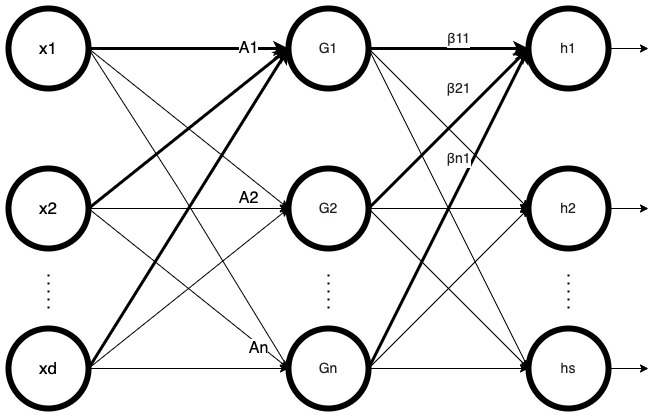
\includegraphics[width=.9\textwidth]{articulo_rrnn_aproximadores_universales/Red-Neuronal-blanco-negro-varias-salidas.jpg}
    \caption{Ejemplo de red neuronal de una capa oculta con $n$ nodos, de dimensión de entrada $d$ y salida $s$.}
    \label{fig:red neuronal-r-h-s}
\end{figure}

Nótese que los vectores $(w_{0i},w_{1 i}, \ldots, w_{r i})$ representan a la aplicación afín 
$A_i((x_1, x_2, \ldots x_r)) = w_{0i} + \sum_{j=1}^d w_{ji} x_j$
con $i \in \{1,\ldots, h\}$ . 

\begin{definicion}[Abstracción de una red neuronal con una capa oculta y múltiple salida] 
    Para cualquier función Borel medible $G$, definida de $\R$ a $\R$ y cualquiera naturales positivo
    $d,s \in \N$ se define a la clase de funciones $\rrnnmc$ como 
    \begin{equation}
        \begin{split}
        \rrnnmc = 
        \{ 
            & h: \R ^d \longrightarrow \R^s, h= (h_1, h_2, \ldots, h_s)  / \quad 
            \\ &
            \text{ con } h_i : \R ^d\longrightarrow \R, 
            h_i(x)=\sum_{j = 1} ^{n_i} (
            \beta_{j i} G(A_{j}(x)) \quad i \in \{1,2,\ldots, s\}, \\
            & x  \in \R ^d, \beta_{j i} \in \R, A_{j}\in \afines,n_i \in \N, i \in \{1,\ldots, s\} 
        \}.
        \end{split}
    \end{equation}
\end{definicion}

\iconoAclaraciones \textcolor{dark_green}{ Nota Blanca: }


Es interesante apreciar que se tiene que 
    \begin{equation} \label{eq:diferencia_conjuntos_multicapa}
        \begin{split}
        \rrnnmc \subsetneq
        \{ 
            & h: \R ^d \longrightarrow \R^s, h= (h_1, h_2, \ldots, h_s)  / \quad 
            \\ &
            h_i \in \rrnn \quad \forall i \in \{1, \ldots, s\}
        \}.
        \end{split}
    \end{equation}
    aunque como veremos en el corolario \ref{corolario:2_6} $\rrnnmc$ es un espacio denso en el conjunto que acabamos de presentar. 
    Si tenemos presente que de acorde a nuestras definiciones una red neuronal $h_i$ viene determinada por un conjunto de funciones afines $A^{(i)}_j$  y escalares $\beta^{(i)_j}$, se daría la igualdad en \refeq{eq:diferencia_conjuntos_multicapa} si imponemos que para cualquier par de redes neuronales $h_k, h_j$ se satisface que $A^{(k)}_i = A^{(j)}_i$. 


No es difícil pensar que su versión generalizada sea: 

\begin{definicion} 
    Dadas las mismas hipótesis que en la definición anterior, se define la siguiente clase de funciones como 
    \begin{equation}
        \begin{split}
            \sum \prod^{d, s}(G) 
            = 
        \{ 
            & f: \R ^d \longrightarrow \R^s, f= (f_1, f_2, \ldots , f_s)  / \quad 
            \\ &
            \text{ con } f_i : \R ^d\longrightarrow \R, 
            f_i(x)=\sum_{j = 1} ^h 
            \left(
            \beta_{j i} \prod_{k=1}^{l_{j i}} G(A_{j i}(x))
            \right)
             \quad i \in \{1,2,\ldots, s\}, \\
            & x \in \R ^d, \beta_{j i} \in \R, A_{j i}\in \afines; h,l_{j i} \in \N 
        \}.
        \end{split}
    \end{equation}
\end{definicion}


% Corolario 2.6  
\begin{corolario}\label{corolario:2_6}
    Los teoremas 
    \ref{teorema:2_3_uniformemente_denso_compactos},
    \ref{teo:2_4_rrnn_densas_M} 
    y los corolarios
    \ref{cor:2_1}, 
    \ref{corolario:2_2_rrnn},
    \ref{corolario:2_3_medida_probabilidad},
    \ref{corolario:2_4_conjunto_finito}
    y 
    \ref{corolario:2_5_función_Booleana}
    permanecen válidos si se sustituye $\rrnn$ por $\rrnnmc$
    ,$\rrnng$ por $\rrnngmc$, 
    los espacios de funciones continuas y medibles por $\fCC$ y $\fMM$ respectivamente.
\end{corolario}

% Nota intuitiva sobre el Corolario 2.6
\marginpar{\maginLetterSize\raggedright
    \iconoAclaraciones \textcolor{dark_green}{ 
        \textbf{Idea clave corolario
        \ref{corolario:2_6}}
    }
}
\marginpar{\maginLetterSize\small
   En esencia, todos los resultados probados hasta ahora para redes 
   neuronales con salida real de dimensión uno son válidos para 
   cualquier tamaño de salida, es decir, \textbf{lo que a nosotros 
   nos interesa podemos aproximar cualquier función medible que 
   vaya entre espacios de dimensión finita}. 
}

% Nota intuitiva sobre la demostración del Corolario 2.6
\marginpar{\maginLetterSize\raggedright
    \iconoAclaraciones \textcolor{dark_green}{ 
        \textbf{Idea clave demostración corolario
        \ref{corolario:2_6}}
    }
}
\marginpar{\maginLetterSize\small
 La demostración del corolario es totalmente constructiva:
si se desea una red neuronal de salida $s\in \N$, 
se construyen de manera independiente $s$ redes neuronales de salida de dimensión uno
(una para cada salida buscada) y las concatenamos haciendo valer cero las conexiones entre nodos que no pertenecieran a las redes de partida.
}
\begin{proof}
    Observemos que todos los teoremas y lemas mencionados basan su tesis
    en la existencia de una red neuronal es decir, que si llamamos según 
    convenga $\mathcal{F}^{d,s}$ a $\rrnnmc$ o $\rrnngmc$ deberemos de 
    encontrar $f \in \mathcal{F}^{d,s}$ que cumplan las respectivas tesis para salidas múltiples. 

    La prueba se construirá por inducción sobre el número de salidas $s$. 

    % Nota nueva hipótesis de optimización del Corolario 2.6
\reversemarginpar
\setlength{\marginparwidth}{\smallMarginSize}

\marginpar{\maginLetterSize\raggedright
     \iconoProfundizar \textcolor{blue}{
        \textbf{Nueva hipótesis de optimización}
    }
}
\marginpar{\maginLetterSize
    \small
    La demostración del corolario nos da una \textbf{técnica constructiva}
    de obtener redes neuronales de varias salidas,
     que puede ser de valía para aplicarla \textbf{como heurística 
     para inicializar los pesos de la red neuronal} como 
     ya apuntábamos en las notas del 
   teorema 
        \ref{teorema:2_5_entrenamiento_redes_neuronales}.
}
\normalmarginpar
\setlength{\marginparwidth}{\bigMarginSize}

    El caso base $s=1$ viene dado por los respectivos teoremas y lemas ya probados.
    Supuesto cierto para $s = n$ veamos que se cumple para $s=n+1$: 
    
    Se quiere encontrar 
    $f = (f_1, f_2, \ldots, f_n, f_{n+1})$ de $n+1$ salidas, 
    por hipótesis de inducción existe $g_n \in \mathcal{F}^{d,n}$ con
     $g_n = (f_1, f_2, \ldots, f_n)$ y con $h_n$ sumandos. Denotamos a los pesos de las transformaciones afines 
     $w_{i j} \in \R$ con 
     $i \in \{0, 1, \ldots , d \}$  y  $j \in \{1, \ldots ,h_n \}$ 
     y $\beta_{ k l} \in \R$ con 
     $k \in \{1, \ldots ,h_n \}$  y  $l \in \{1, \ldots ,n \}.$

    También existe $g_1 \in \mathcal{F}^{d,1}$ cumpliendo que
    $g_1 = f_{n+1}$ con $h_1$ sumandos en la capa oculta
    y pesos  
    ${w'}_{i j} \in \R$ con 
     $i \in \{0, 1, \ldots , d \}$  y  $j \in \{1, \ldots , h_1 \}$ 
     y ${\beta '}_{ k l} \in \R$ con 
     $k \in \{1, \ldots , h_1 \}$  y  $l = {n+1}$
     (Ver figura \ref{fig:red neuronal-r-h-s} para orientarse en la notación tomada).
     
    Considerando $f$ compuesta por $h_n + h_1$ sumandos y donde sus pesos son los siguientes:

    El peso $\tilde{w}$ de las funciones afines: 
    Para cuales quiera 
    $i \in \{0, 1, \ldots  , d \}$  y  
    $j \in \{1, \ldots , h_n, h_{n} + 1, \ldots, h_n + h_1\}$  determinaremos la siguiente casuística
    \begin{enumerate}
        \item Si $1 \leq j \leq h_n$ entonces $\tilde{w}_{i j} = w_{i j}.$
        \item Si $h_n < j \leq h_n + h_1$ entonces $\tilde{w}_{i j} = w_{i (j-h_n)}.$
    \end{enumerate}

    Para los pesos $\tilde{\beta}$, para cualquier
    $k \in \{1, \ldots , h_n, h_{n} + 1, \ldots, h_n + h_1\}$ y  
    $l \in \{1, \ldots ,  n+1 \} :$ 
    \begin{enumerate}
        \item Si $k \in \{1, \ldots ,  h_n \}$ y $l \in \{1, \ldots , n\}$ 
        entonces $\tilde{\beta}_{k l} = \beta_{k l}.$
        \item Si $k \in \{1, \ldots , h_n \}$ y $l=n+1$ 
        entonces $\tilde{\beta}_{k l} = 0.$
        \item Si $k \in \{h_{n} + 1, \ldots, h_n + h_1 \}$ 
        y $l \in \{1, \ldots , n\}$ 
        entonces $\tilde{\beta}_{k l} = 0.$
        \item Si $k \in \{h_{n} + 1, \ldots, h_n + h_1 \}$ 
        y $l=n+1$ 
        entonces 
        $\tilde{\beta}_{k l} = {\beta '}_{(k- h_n) l}.$
    \end{enumerate}

    Notemos que $f=(f_1, f_2, \ldots, f_n, f_{n+1})$, es decir $f \in \mathcal{F}^{d,s}$, y que para cada teorema o lema
    cada una de las proyecciones de $f$ cumple la tesis, es decir $f$ cumple lo buscado. 
\end{proof}

\subsubsection*{ Conclusión sobre el teorema anterior}  
A la vista de la demostración constructiva se nos acaba de decir de manera indirecta que si queremos construir una red neuronal 
a partir de un tamaño de entrenamiento $E$ y de salida de dimensión $s$, 
con una red neuronal de $E \times s$ neuronas en la ocultas será suficiente y para este caso la reflexión expuesta en la sección \ref{subsection:reflexión_sobre_número_de_neuronas} es idéntica. 



